\mode*
% Plataformas e instituciones:
% USA-MIT-Tedrake-TODDLER
% RABBIT-EMARO-Universidad de Nantes-
\section[Justificaci\'on]{Justificaci\'on}
\label{sec:justify}

\mode<presentation>{
\begin{frame}
  \frametitle{Por qu\'e esta investigaci\'on?}
  \framesubtitle{Universidades, Institutos, Centros y Laboratorios trabajando en Rob\'otica B\'ipeda}
  \begin{center}
    \includegraphics[height=7cm]{../images/BipedInstitutesAndUniversities.png}
  \end{center}
\end{frame}
\begin{frame}
  \frametitle{Por qu\'e esta investigaci\'on?}
  \framesubtitle{Algunas plataformas b\'ipedas}
  \begin{center}
    \includegraphics[height=6.5cm]{../images/BipedPlatforms.png}
  \end{center}
\end{frame}
\begin{frame}[label=def_multi]
  \frametitle{Por qu\'e esta investigaci\'on?}
  \framesubtitle{Trabajo multidisciplinario}
  \begin{center}
    \only<1-6,7>{
      \only<1-6>{\vspace{-2.0cm}}
      \only<7>{\vspace{-0.3cm}}
      \begin{columns}[c]
        \begin{column}{3cm}
          \only<1>{\setbeamercolor{postit}{fg=white,bg=red!50!black}}
          \only<2-7>{\setbeamercolor{postit}{fg=white,bg=red}}
          \hyperlink{exp_embebidos}{
          \begin{beamercolorbox}[sep=0.5em,wd=3cm,rounded=true,center,shadow=true]{postit}
            \only<1>{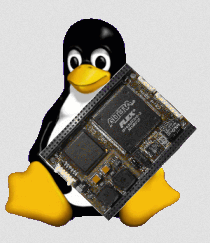
\includegraphics[height=1.5cm]{../images/ThemeEmbedded.png}\\}
            \only<2-6>{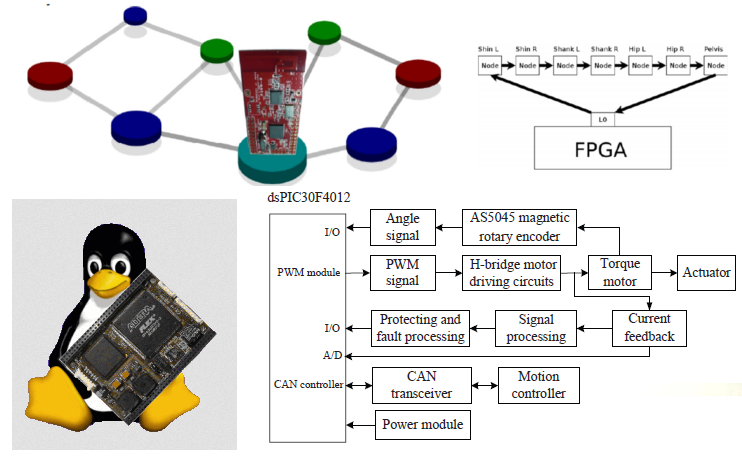
\includegraphics[height=1.5cm]{../images/ShortEmbedded.png}\\}
            \textbf{Sistemas Embebidos}
          \end{beamercolorbox}}
        \end{column}
        \begin{column}{3cm}
          \only<1-2>{\setbeamercolor{postit}{fg=white,bg=yellow!70!black}}
          \only<3-7>{\setbeamercolor{postit}{fg=white,bg=yellow}}
          \hyperlink{exp_biomecanica}{
          \begin{beamercolorbox}[sep=0.5em,wd=3cm,rounded=true,center,shadow=true]{postit}
            \only<1-2>{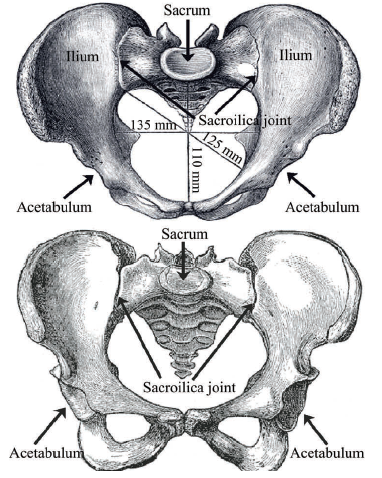
\includegraphics[height=1.5cm]{../images/ThemeBiomechanics.png}\\}
            \only<3-6>{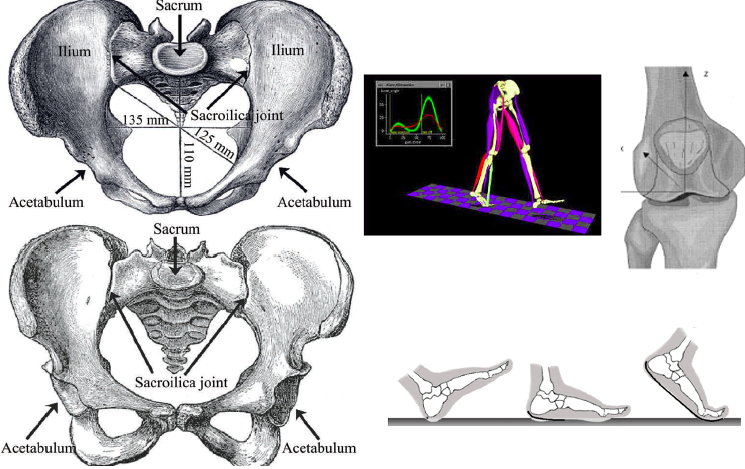
\includegraphics[height=1.5cm]{../images/ShortBiomechanics.png}\\}
            \textbf{Biomec\'anica}
          \end{beamercolorbox}}
        \end{column}
        \begin{column}{3cm}
          \only<1-3>{\setbeamercolor{postit}{fg=white,bg=blue!50!black}}
          \only<4-7>{\setbeamercolor{postit}{fg=white,bg=blue}}
          \hyperlink{exp_mecanismos}{
          \begin{beamercolorbox}[sep=0.5em,wd=3cm,rounded=true,center,shadow=true]{postit}
            \only<1-3>{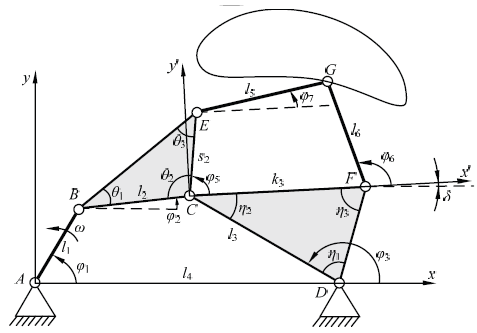
\includegraphics[height=1.5cm]{../images/ThemeMechanisms.png}\\}
            \only<4-6>{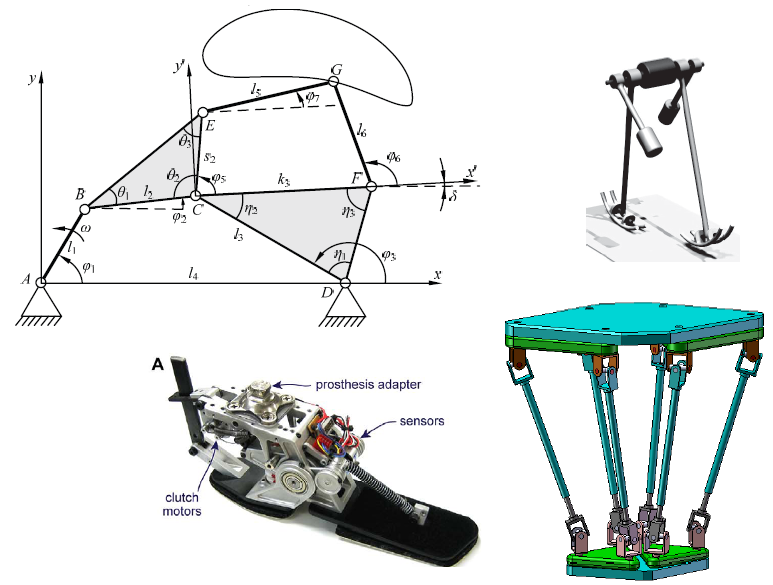
\includegraphics[height=1.5cm]{../images/ShortMechanisms.png}\\}
            \textbf{Modelado y Mecanismos}
          \end{beamercolorbox}}
        \end{column}
      \end{columns}
      \vspace{1.0cm}
      \begin{columns}[c]
        \begin{column}{3cm}
          \only<1-4>{\setbeamercolor{postit}{fg=white,bg=black}}
          \only<5-7>{\setbeamercolor{postit}{fg=white,bg=white!50!black}}
          \hyperlink{exp_computacion_flexible}{
          \begin{beamercolorbox}[sep=0.5em,wd=3cm,rounded=true,center,shadow=true]{postit}
            \textbf{C. Flexible y Optimizaci\'on}
            \only<1-4>{\\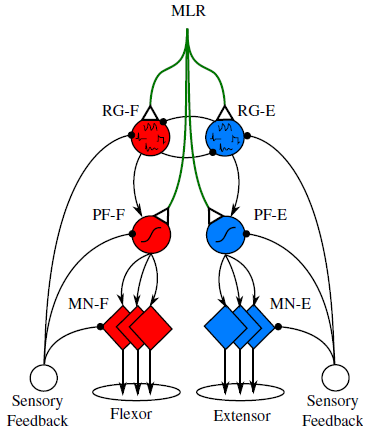
\includegraphics[height=1.5cm]{../images/ThemeSoftComputing.png}}
            \only<5-6>{\\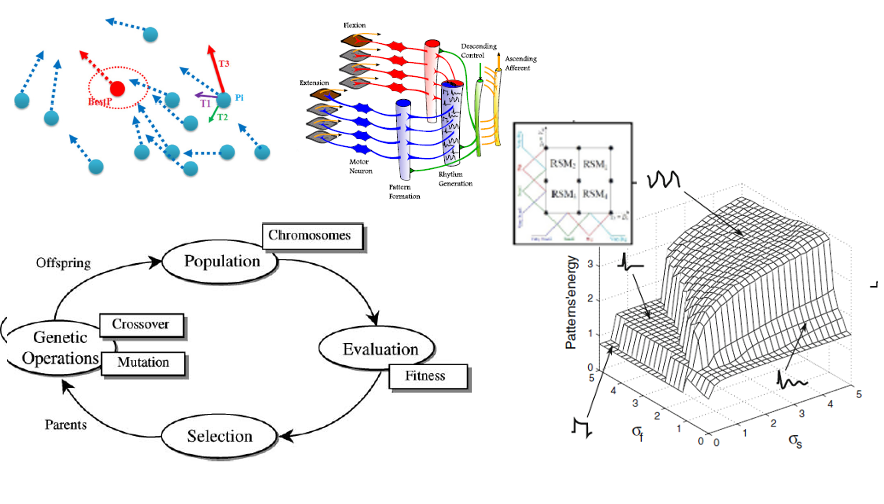
\includegraphics[height=1.5cm]{../images/ShortSoftComputing.png}}
          \end{beamercolorbox}}
        \end{column}
        \begin{column}{3cm}
          \only<1-5>{\setbeamercolor{postit}{fg=white,bg=green!50!black}}
          \only<6-7>{\setbeamercolor{postit}{fg=white,bg=green}}
          \hyperlink{exp_control}{
          \begin{beamercolorbox}[sep=0.5em,wd=3cm,rounded=true,center,shadow=true]{postit}
            \textbf{Control y Sis. Din\'amicos}
            \only<1-5>{\\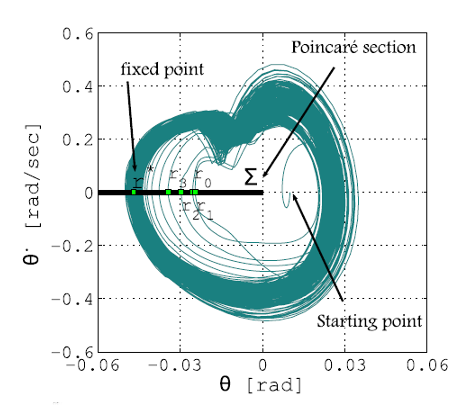
\includegraphics[height=1.5cm]{../images/ThemeControl.png}}
            \only<6-6>{\\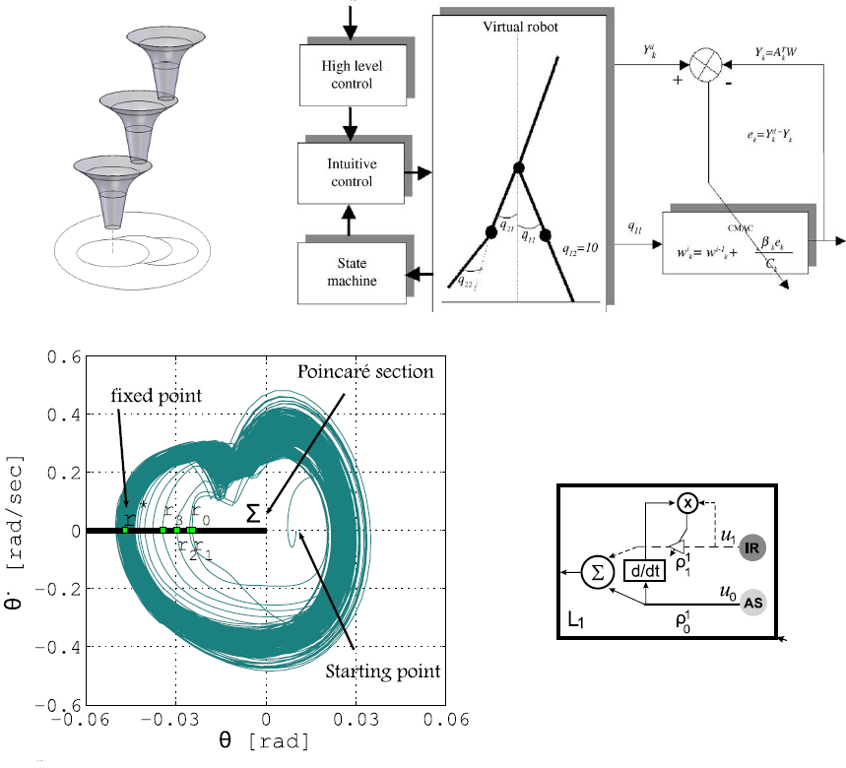
\includegraphics[height=1.5cm]{../images/ShortControl.png}}
          \end{beamercolorbox}}
        \end{column}
      \end{columns}
      \only<1-6>{\vspace{-4.6cm}}
      \only<7>{\vspace{-3.1cm}}
      \hspace{-0.1cm}
      \setbeamercolor{postit}{fg=white,bg=blueun}
      \begin{beamercolorbox}[sep=0.5em,wd=4.0cm,rounded=true,center]{postit}
        \textbf{\Large\textcolor{white}{ROB\'OTICA B\'IPEDA}}
      \end{beamercolorbox}
    }
%    \only<2>{\textbf{\textcolor{blueun}{Sistemas Embebidos}}\\
%    \includegraphics[height=6.5cm]{../images/Embedded.png}}
%    \only<3>{\textbf{\textcolor{blueun}{Biomec\'anica}}\\
%    \includegraphics[height=5.8cm]{../images/Biomechanics.png}}
%    \only<4>{\textbf{\textcolor{blueun}{Modelado de sistemas mec\'anicos y s\'intesis de mecanismos}}\\
%    \includegraphics[height=6.0cm]{../images/Mechanisms.png}}
%    \only<5>{\textbf{\textcolor{blueun}{Optimizaci\'on, computaci\'on flexible e IA}}\\
%    \includegraphics[height=6.0cm]{../images/SoftComputing.png}}
%    \only<6>{\textbf{\textcolor{blueun}{Control}}\\
%    \includegraphics[height=6.5cm]{../images/Control.png}}
  \end{center}
\end{frame}
\begin{frame}
  \frametitle{Por qu\'e esta investigaci\'on?}
  \framesubtitle{Algunos aspecto para la justificaci\'on}
  \quad\hspace{-0.8cm}\makebox{
    \begin{columns}[T]
      \small
      \begin{column}{6cm}
        \begin{enumerate}
        \item Como ayuda de la proliferaci\'on
          \only<2-6>{
            \begin{itemize}\scriptsize
            \item<2-> Bajo costo
            \item<3-> Didacticos
            \item<4-> Modularidad
            \item<5-> Prototipado rapido
            \item<6-> Metodologia de dise\~no
            \end{itemize}
          }
        \item<7-> Motivaci\'on personal
        \item<8-> Posibles productos y soluciones
          \only<9-13>{
            \begin{itemize}\scriptsize
            \item<9-> Teleoperaci\'on
            \item<10-> Manufactura, transporte y ensambles
            \item<11-> Movilidad en cuadrapl\'ejicos, pr\'otesis y caminata pasiva
            \item<12-> Educaci\'on, cursos y materias
            \item<13-> Entretenimiento e IA
            \end{itemize}
          }
        \item<14-> Viabilidad
          \only<15->{
            \begin{itemize}\scriptsize
            \item<15-> Recursos f\'isicos
            \item<16-> Profesores, grupos de investigaci\'on y materias
            \item<17-> Concursos para recursos economicos y de financiaci\'on
            \item<18-> Relaciones con grupos internacionales de investigaci\'on
            \item<19-> Experiencia del director de investigaci\'on en el tema
            \item<20-> Experiencia del investigador en el proyecto
            \end{itemize}
          }
        \end{enumerate}
      \end{column}
      \begin{column}{4cm}
        % \fbox{
        \parbox[c][7cm][c]{4cm}{
          \only<1-4>{
            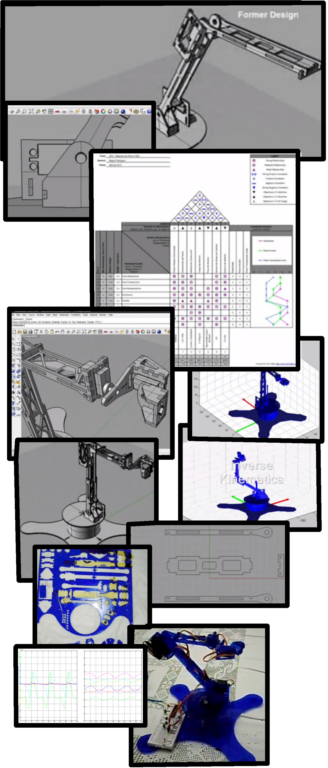
\includegraphics[height=7cm]{../images/RobotMR1_0.png}
          }
          \only<5>{
            %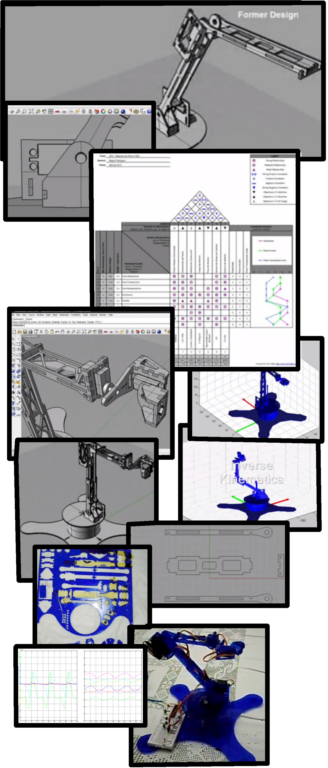
\includegraphics[height=7cm]{../images/RobotMR1_0.png}
            \animategraphics[height=7cm,autoresume,autoplay,loop]{2}{../images/RobotMR1_}{0}{12}
          }
          \only<6>{
            %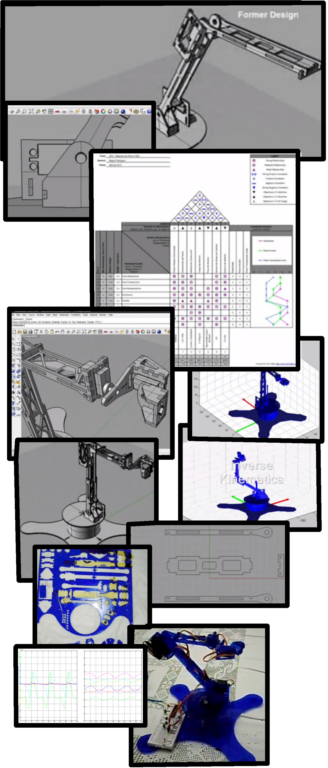
\includegraphics[height=7cm]{../images/RobotMR1_0.png}
            \movie[width=3cm,height=7cm,externalviewer]{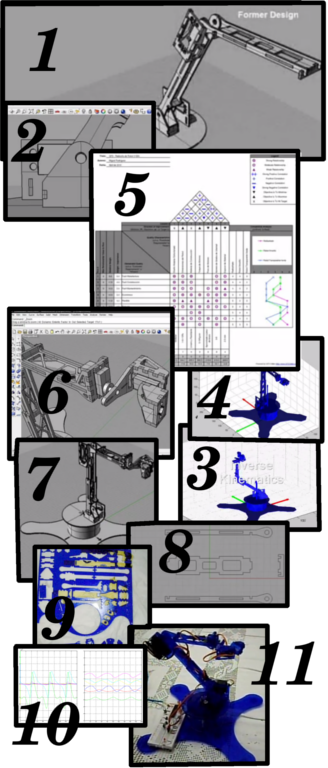
\includegraphics[height=7cm]{../images/RobotMR1_12.png}}{../videos/RobotMR1.flv} 
          }
          \only<7>{
            \scriptsize
            \begin{center}
              \includegraphics[height=7.0cm]{../images/SomeThingsByMeSumary.png}
            \end{center}
          }
          \only<9>{
            \scriptsize
            Teleoperaci\'on
            \begin{center}
              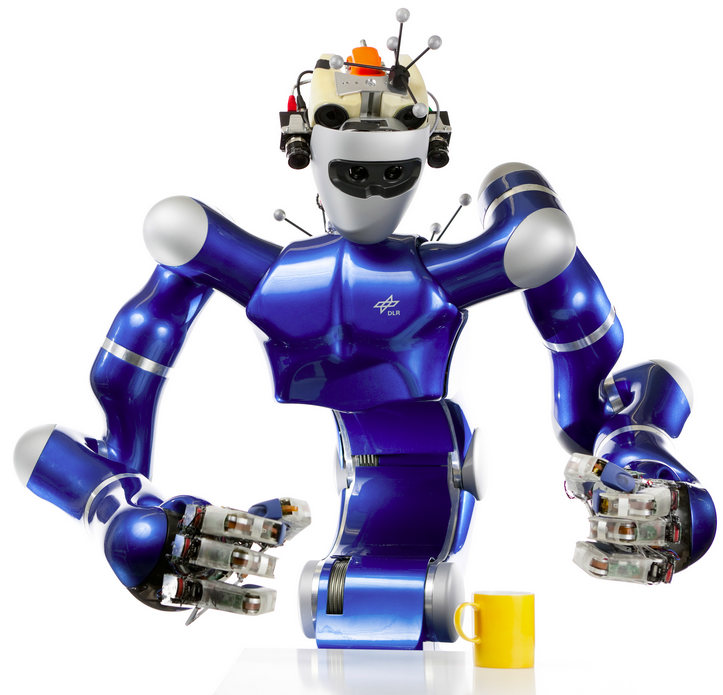
\includegraphics[width=4.0cm]{../images/Teleoperacion.png}
            \end{center}
          }
          \only<10>{
            \scriptsize
            Transporte
            \begin{center}
              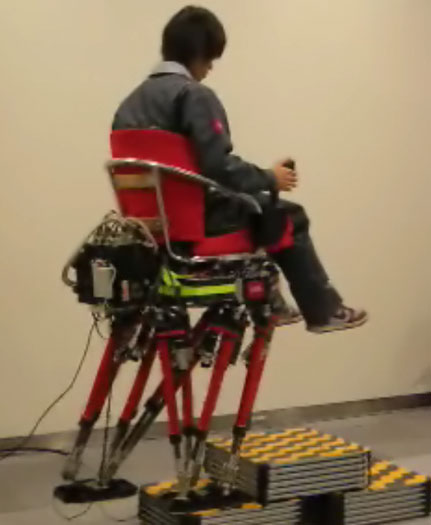
\includegraphics[width=4.0cm]{../images/Transporte.png}
            \end{center}
          }
          \only<11>{
            \scriptsize
            Biomec\'anica
            \begin{center}
              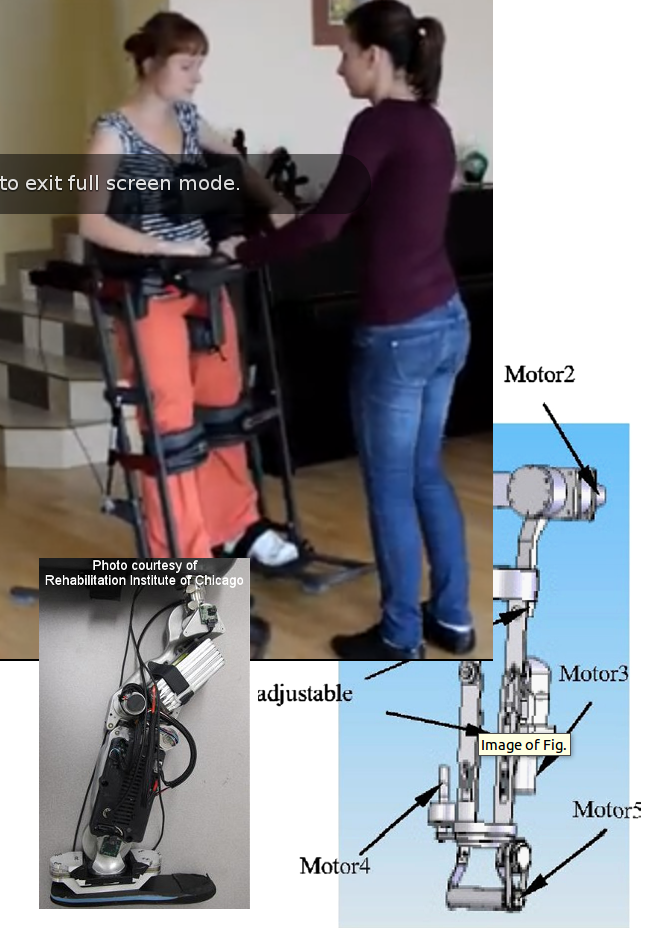
\includegraphics[width=4.0cm]{../images/ProsthesisAndPhysiotherapy.png}
            \end{center}
          }
          \only<12>{
            \scriptsize
            Educaci\'on
            \begin{center}
              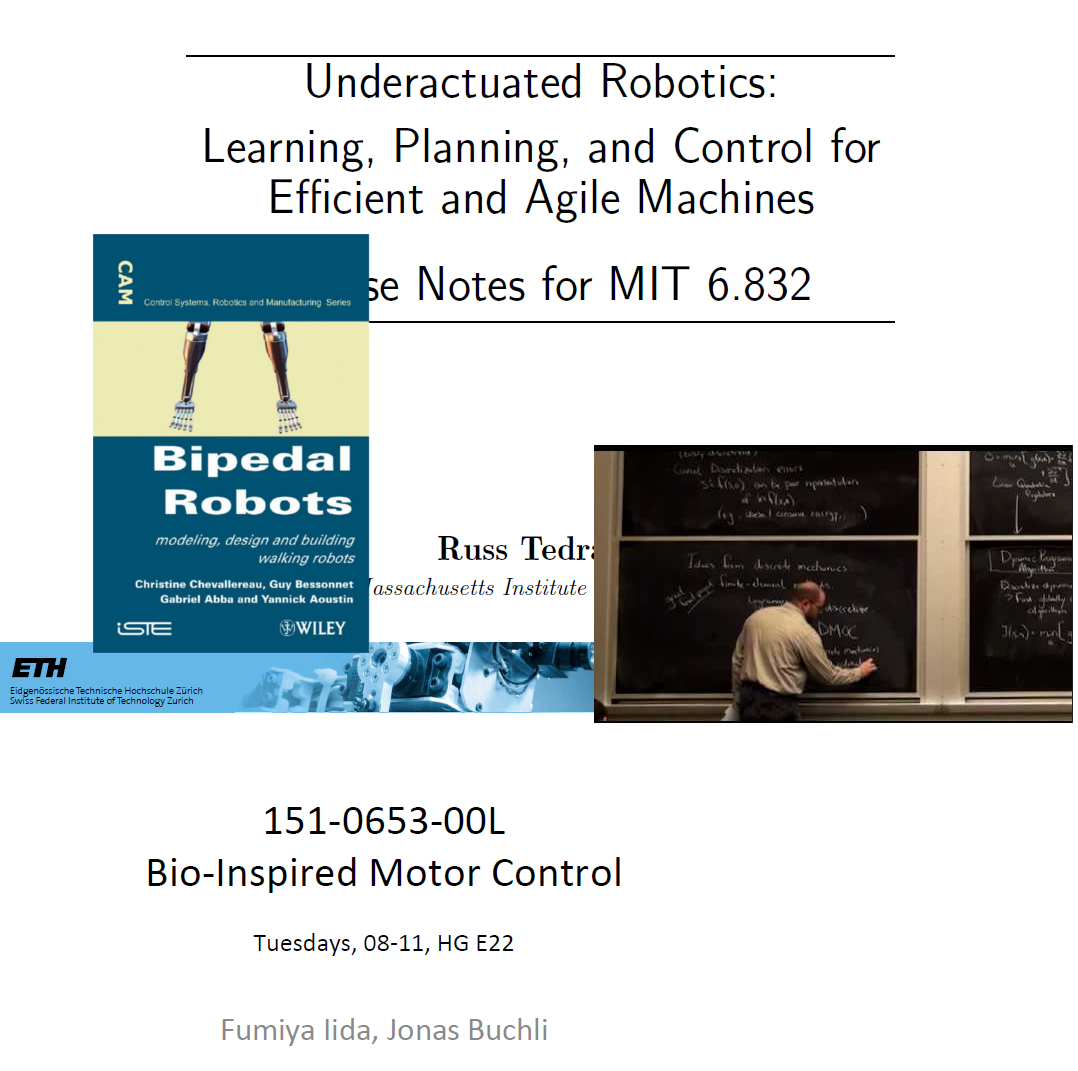
\includegraphics[width=4.0cm]{../images/Educacion.png}
            \end{center}
          }
          \only<13>{
            \scriptsize
            Entretenimiento
            \begin{center}
              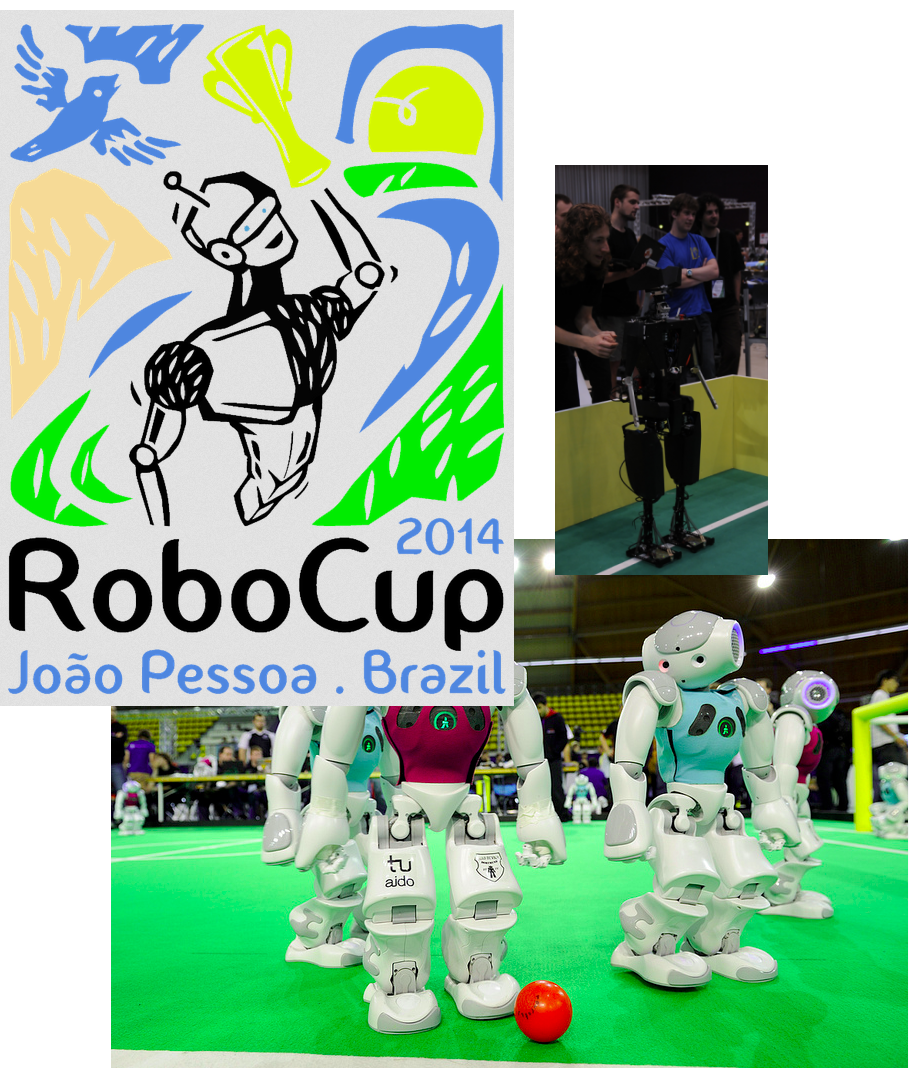
\includegraphics[width=4.0cm]{../images/Entretenimiento.png}
            \end{center}
          }
          \only<15>{
            \scriptsize
            \begin{itemize}
            \item CNC
            \item Impresoras 3D
            \item Software CAD-CAM-CAE
            \item Laboratorios con plataformas
            \end{itemize}
          }
          \only<16>{
            \scriptsize
            \begin{itemize}
            \item Din\'amica de robots (R. Ram\'irez)
            \item Biomec\'anica (D. Garzon)
            \item Sistemas embebidos (C. Camargo)
            \item Control de robots (J. Sofrony)
            \item Aprendizaje de m\'aquina (F. Gonz\'alez)
            \item Optimizaci\'on (A. Tovar)
            \item Computaci\'on flexible (L.F Ni\~no)
            \item Inteligencia Artificial (J. G\'omez)
            \end{itemize}
          }
          \only<18>{
            \scriptsize
            \begin{itemize}
            \item Justin DLR (M. Roa)
            \item Robonaut 2 GM-NASA (L. Barajas)
            \item Walking Dynamics Conferences
            \end{itemize}
          }
          \only<19>{
            \scriptsize
            \begin{center}
              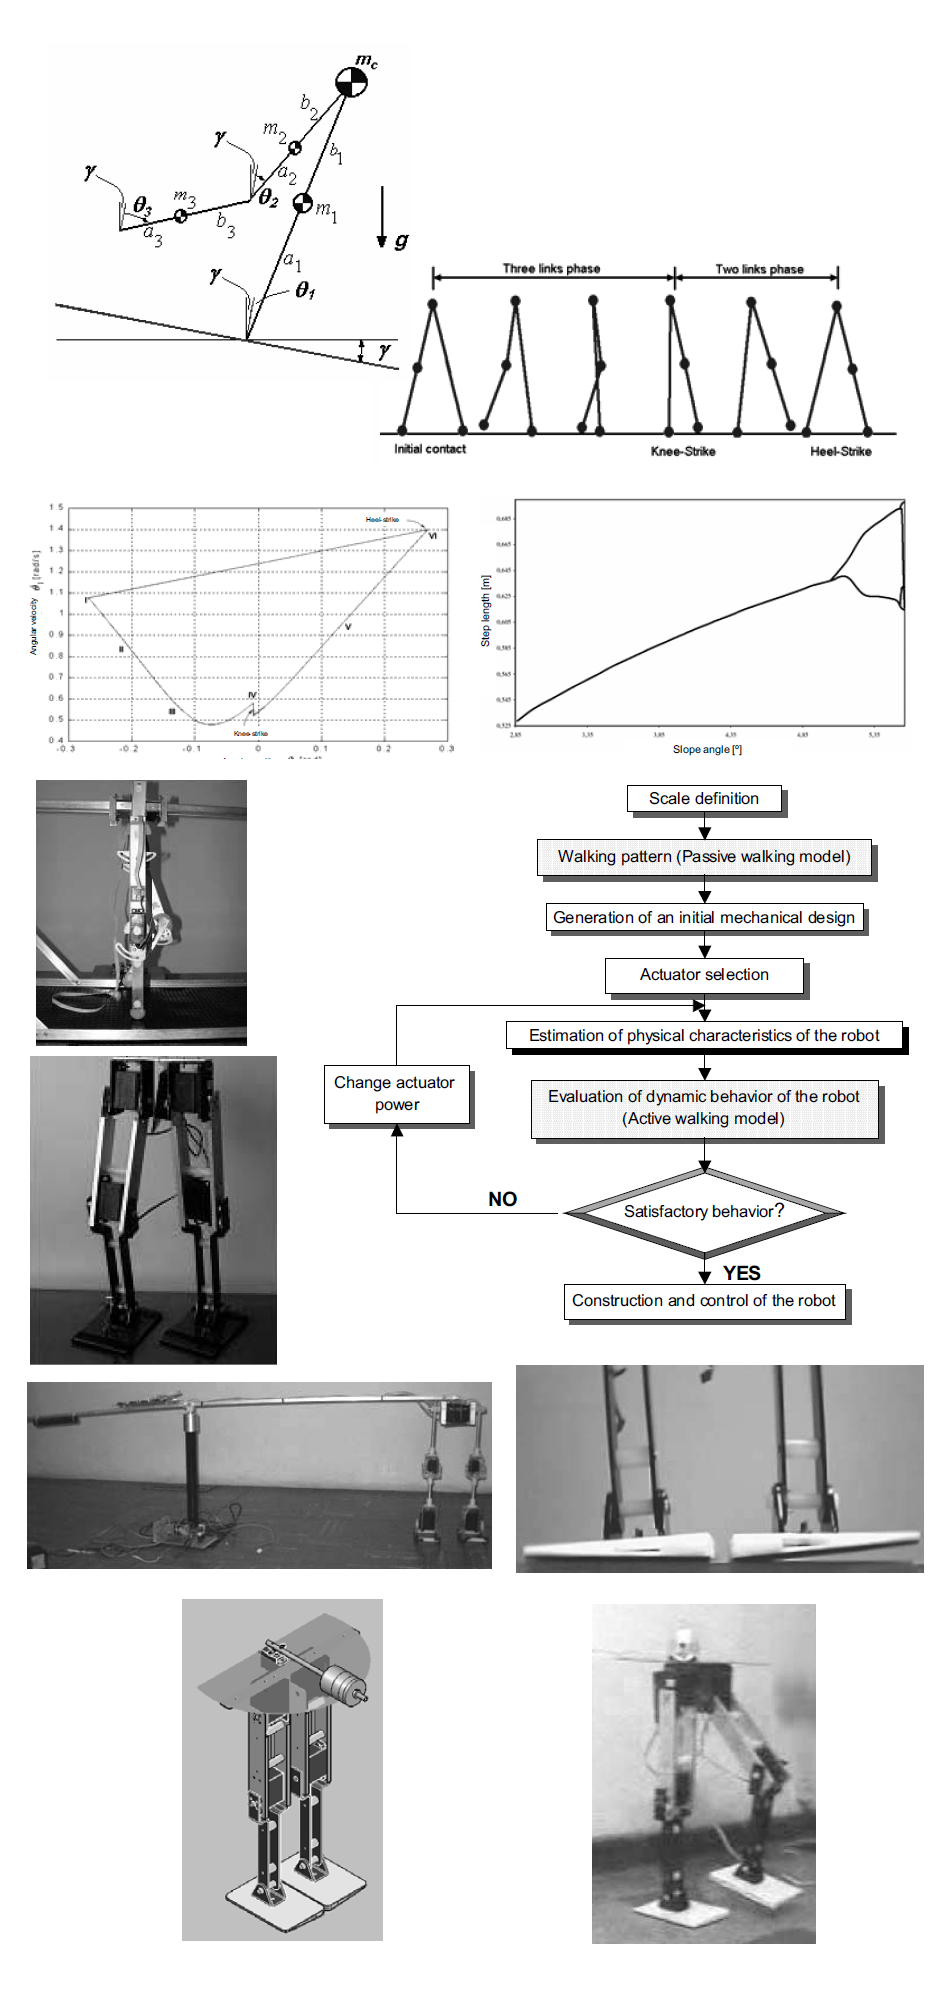
\includegraphics[height=7.0cm]{../images/UNROCA.png}
            \end{center}
          }
          \only<20>{
            \scriptsize
            \begin{center}%P1(120,360),P2(1110,530)
              %\includegraphics[height=7cm]{../images/SomeThingsByMe_0.png}
              \animategraphics[height=7cm,autoresume,autoplay,loop]{1}{../images/SomeThingsByMe_}{1}{5}
            \end{center}
          }
        }
        % }
      \end{column}
    \end{columns}
  }
  \only<18>{\vspace{-2.0cm}
    \begin{center}
      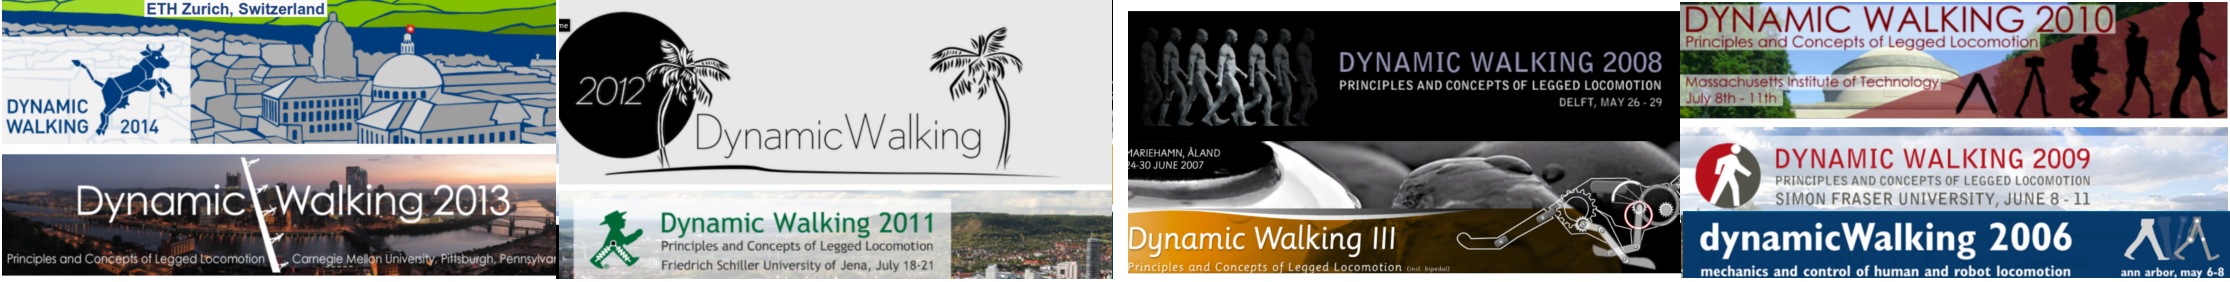
\includegraphics[width=10.0cm]{../images/DynamicWalkingConferences.png}
    \end{center}
  }
\end{frame}
\begin{frame}
  \frametitle{Por qu\'e esta investigaci\'on?}
  \begin{itemize}
  \item Curso Posgrado de Camidadores y L\'inea de investigaci\'on: Modelado, Control y Planeaci\'on.
  \item Vukobratovic, McGeer, Goswami, Kuo, Tedrake, Collins, Ruina, Wisse, Chevallereau, Westervelt, Spong, Gregg, Ijspeert
  \item Arquitecturas paralela en la rob\'otica b\'ipeda, dise\~no de rodilla, tobillo, talon-planta-toe.
  \item Generaci\'on de locomocion cuadrapejica y rehabilitaci\'on.
  \item Aprendizaje por refuerzo.
  \item Estabilidad usando Lyapunov y \'arboles de LQR.
  \item Central pattern generators.
  \item Rimless-Wheel, Inertial-Wheel, Compass-Gait. 
  \item MIKE, MAX, DENISE, Toddler-MIT.
  \item RABBIT, ERNIE.
  \item Zero-Moment-Point.
  \item Passive-Dynamics y Control de trayectorias.
  \item Capture-points.
  \end{itemize}
\end{frame}
}
Buscando una proliferaci\'on robusta de la rob\'otica en el pa\'is a nivel tecnol\'ogico y del conocimiento de esta \'area, se da acontinuaci\'on la justificaci\'on de este proyecto de investigaci\'on, propuesta que se ve acotada a ser trabajada en el mundo de la r\'obotica de caminadores.  Las tendencias a nivel mundial que se desarrollan en este tema actu\'almente, crecen cada d\'ia a pasos agigantados provocados por cientos de grupos de investigaci\'on pertenecientes a Universidades, Institutos, Centros y Laboratorios en todo el mundo.\par
Aunque la Universidad Nacional de Colombia ya comenz\'o sus investigaciones en el \'area con interesantes resultados\cite{M2005,M2005a,Roa2006,Heredia2007}, en donde se han construido lazos por medio de investigadores, profesores y estudiantes de la Universidad con otros grupos de vital importancia a nivel mundial en el \'area, como es el caso de \cite{Englsberger2011,Ott2011,M2013}. Desde hace unos siete a\~nos no se han desarrollado proyectos importantes en el \'area de caminadores.\par
El campo de la rob\'otica b\'ipeda ha superado algunos problemas y han surgido unos nuevos, en donde las soluciones encontradas han sido generadas integrando m\'ultiples fuentes de conocimiento, en \'areas como: los sistemas embebidos\cite{Barker2010,Pan2010,Kimm2012,Wang2011,Amir2013}, la biomec\'anica\cite{Mahmoodi2013,Lim2014,Wu2013,Aoustin2013,Chiang2013,Xiang2010,Hobon2014}, el modelado de sistemas mec\'anicos\cite{Chiang2013}, la s\'intesis de mecanismos\cite{Li2008,Aoustin2013,Wu2013a,Xu2013,Hobon2014}, la optimizaci\'on\cite{Xiang2010,Lim2014,Kherici2014,Mahmoodabadi2014}, la computaci\'on flexible\cite{Wang2013,Kherici2014,Mahmoodabadi2014}, la inteligencia artificial\cite{Treesatayapun2014,Yuan2014,Wu2014,Wang2013} y el control\cite{Dou2013,Treesatayapun2014,Yuan2014,Wu2014}.\par
A continuaci\'on se organizan algunos aspectos que forman parte de la justificaci\'on:
\begin{itemize}
\item Se requiere de dise\~nos de caminadores de bajo costo, funcionales, did\'acticos, modulares y de prototipado r\'apido especiales para la ense\~nanza de la rob\'otica, el control y los sistemas distribuidos, y la comprobaci\'on de teor\'ias de control de varias capas de locomoci\'on.
\item Inter\'es personal por el tema, ya que despierta toda mi curiosidad y me apasiona, es un \'area en la que aplica la Mecatr\'onica en todo su poder. Involucrando la electr\'onica, la mec\'anica, la teor\'ia de la computaci\'on, la programaci\'on y su experimento debe resultar en algo \'util y real.
\item \emph{Aplicabilidad:} La aplicaci\'on de los conocimientos que se obtengan servir\'an la soluci\'on de problemas y productos en \'areas como: la industria de los manipuladores en el \'area de la teleoperaci\'on\cite{Treesatayapun2014,M2013}, la manufactura en el transporte de materiales y ensambles\cite{Roy2013}, la fabricaci\'on de pr\'otesis\cite{Roa2006}, la fisioterapia\cite{Kang2013}, la educaci\'on como herramienta did\'actica y motivacionial\cite{Ishida2004}, el entretenimiento, el area de la teor\'ia de juegos y agentes inteligenes como es el caso del futbol de robots ademas de afianzar la l\'inea de investigaci\'on en al Universidad ante nuevos retos\cite{Ishida2004}.
\item \emph{Viabilidad:} El proyecto y la Universidad cuenta con: 
  \begin{enumerate}[1)]
  \item Recursos f\'isicos como centros de mecanizado, impresoras 3D, salas CAD con herramientas computacionales como: Matlab, Ansys, SolidWorks, ademas de laboratorias con distintas plataformas rob\'oticas funcionales.
  \item Profesores, grupos de investigaci\'on y materias bien formadas en temas pertinentes para esta investigaci\'on como Din\'amica de Robots, Biomec\'anica, Sistemas Embebidos, Control Avanzado, Computaci\'on Flexible, Aprendizaje de m\'aquina, Inteligencia Artificial, Optimizaci\'on, Manufactura Computalizada, Redes de comunicaci\'on y otras m\'as.
  \item  Mecanismos y concursos tanto internos como externos a la Universidad para obtener recursos econ\'omicos para fabricaci\'on de prototipos y adquisici\'on de: sensores, actuadores, herramientas, materiales e insumos.
  \item Posibles lazos con importantes grupos de investigaci\'on e investigadores como lo son Justin DLR(por medio de PhD Maximo Roa) y Robonaut 2 GM-NASA(por medio de PhD. Leandro Barajas).
  \item Experiencia del director de investigaci\'on de esta propuesta con aproximadamente 20 a\~nos de experiencia, con trabajos en el tema como \'articulos\cite{Heredia2007}, cap\'itulos de libros\cite{M2005,M2005a}, direcciones de tesis de pregrado y posgrado, y materias de pregrado como de posgrado en la Universidad.
  \item Experiencia y perfil del investigador en el tema de este proyecto, con 8 a\~nos de experiencia en temas de rob\'otica serial y paralela, con trabajos como: direcci\'on de tesis de pregrado\cite{Cortes2009,Valencia2009,Barragan2009,Silva2009}, art\'iculos\cite{Castillo2007}, librer\'ias\cite{Castillo2008}, desarrollo de software de simulaci\'on\cite{Castillo2010} y la materia de pregrado de Rob\'otica en la Universidad Nacional de Colombia durante tres a\~nos y medio consecutivos. Adem\'as de experiencia en temas de automatizaci\'on, control e instrumentaci\'on en la industria y la academia.
  \end{enumerate}
\end{itemize}

